\documentclass[tikz, preview]{standalone}

\usepackage{amsfonts, amsthm, amssymb, amsmath, stmaryrd, etoolbox}
\usepackage{tikz}
\usetikzlibrary{matrix,arrows}

\begin{document}
\[
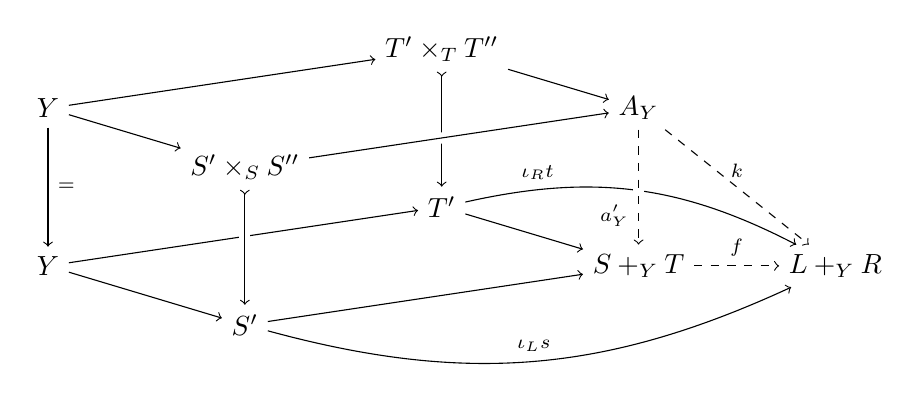
\begin{tikzpicture}
\node (Yt) at (0,2) {$Y$};
\node (Yb) at (0,0) {$Y$};
\node (Spb) at (2.5,1.25) {$S'\times_SS''$};
\node (S') at (2.5,-0.75) {$S'$};
\node (Tpb) at (5,2.75) {$T'\times_TT''$};
\node (T') at (5,0.75) {$T'$};
\node (Ay) at (7.5,2) {$A_Y$};
\node (SyT) at (7.5,0) {$S+_YT$};
\node (LyR) at (10,0) {$L+_YR$};
%
\draw [->] (Yt) edge[] (Tpb);
\draw [->] (Yt) edge[] (Spb);
\draw [font=\scriptsize,->] (Yt) edge node[right] {$=$} (Yb);
\draw [->] (Yb) edge[] (T');
\draw [->] (Yb) edge[] (S');
\draw [->] (Tpb) edge[] (Ay);
\draw [>->] (Tpb) edge[] (T');
\draw [font=\scriptsize,->] (Ay) edge[dashed] node[above] {$k$} (LyR);
\draw [->] (S') edge[] (SyT);
\draw [font=\scriptsize,->] (S') edge[bend right=20] node[above] {$\iota_Ls$} (LyR);
\draw [font=\scriptsize,->] (T') edge[bend left=20] node[above,pos=.2] {$\iota_Rt$} (LyR);
\draw [->] (T') edge[] (SyT);
\draw [font=\scriptsize,->] (SyT) edge[dashed] node[above] {$f$} (LyR);
%
\draw [->] (Spb) edge[white,line width=4pt] (Ay);
\draw [->] (Spb) edge[] (Ay);
\draw [>->] (Spb) edge[white,line width=4pt] (S');
\draw [>->] (Spb) edge[] (S');
\draw [->] (Ay) edge[white,line width=4pt] (SyT);
\draw [font=\scriptsize,->] (Ay) edge[dashed] node[pos=0.75,left] {$a'_Y$} (SyT);
\end{tikzpicture}
\]
\end{document}
